\chapter{Implementation Details}
This chapter describes how the system was built. Section~5.1 states the development environment. Section~5.2 describes the datasets and their sources. Section~5.3 describes the model implementation and how the client and service share it. Section~5.4 records the evaluation metrics and the steps taken for reproducibility. Section~5.5 presents the delivered application.

\section{Development Environment}
The project is a single repository with two overlapping workspaces. A pnpm workspace holds the TypeScript client and the shared client-side engines, and a uv workspace holds the Python packages, the intelligence service, and the offline research code. The two coexist so that the research code can import the same Python engines the service runs, which keeps the evaluated code and the shipped code identical. Table~\ref{tab:tools} lists the environment.

\begin{table}[htbp]
\centering
\footnotesize
\caption{Development environment: tools and libraries.}
\label{tab:tools}
\begin{tabular}{p{4.0cm} p{8.4cm}}
\toprule
\textbf{Concern} & \textbf{Technology} \\
\midrule
Client language and build & TypeScript, Vite, pnpm workspace \\
Client UI & React~19 \\
Local-first storage & Dexie over IndexedDB \\
Intelligence service & Python~3.12, FastAPI, Uvicorn \\
Scientific stack & NumPy, SciPy \\
Service authentication & PyJWT, verifying Supabase-issued tokens \\
Containerisation & Docker via Colima \\
Python workspace & uv \\
JavaScript testing & Vitest, fast-check (property tests), Playwright (end-to-end) \\
Python testing and linting & pytest, ruff \\
Backend and hosting & Supabase (auth, database, storage), Vercel \\
\bottomrule
\end{tabular}
\end{table}

\section{Datasets and Their Sources}
Because a single learner's real log cannot supply a known ground truth, the comparison in Chapter~6 is run on synthetic data whose properties are planted and therefore known. Table~\ref{tab:datasets} lists the datasets and the role each plays.

The synthetic generator produces study histories in which the learner's true pace, the timing and size of any regime shift, and the completion behaviour are set explicitly. So that the synthetic regime resembles real behaviour rather than an arbitrary one, its parameters were calibrated against the Open University Learning Analytics Dataset (OULAD), a large public dataset of learner activity. The OULAD is used only to calibrate the generator's realism; it is not used as a direct benchmark. A revised generator regime models the booking interaction pattern introduced by the redesign of Section~4.4, and the selected models were re-checked against it. Real single-learner logs are reserved for the longitudinal validation planned in Phase~II and are not used in Phase~I.

\begin{table}[htbp]
\centering
\footnotesize
\caption{Datasets used in Phase~I and their sources.}
\label{tab:datasets}
\begin{tabular}{p{3.6cm} p{3.8cm} p{5.0cm}}
\toprule
\textbf{Dataset} & \textbf{Source} & \textbf{Role} \\
\midrule
Synthetic study histories & Generated in-repository & Primary ground truth for the component comparison; plants pace, shifts, and learner archetypes \\
OULAD & Public (Open University) & Calibrates the synthetic generator's realism regime; not a direct benchmark \\
Revised (decoupled) regime & Generated in-repository & Re-validates the selected models under the booking interaction model \\
Real single-learner log & The candidate's own sessions & Phase-II longitudinal validation; not used in Phase~I \\
\bottomrule
\end{tabular}
\end{table}

\section{Model Implementation}
The algorithms are implemented once in behaviour and twice in code. The client-side engines are written in TypeScript, and a Python mirror of each engine is exposed through the intelligence service. The two implementations are kept aligned by a golden-fixture parity harness: the TypeScript engines emit reference inputs and outputs, and a Python test replays each input and asserts numeric equality to a tight tolerance. The shared numeric constants, such as the Bayesian prior, the CUSUM slack and threshold factors, and the Gaussian-process length scale, are held identical on both sides.

The split between client and service follows the architecture of Figure~\ref{fig:arch-revised}. Computation that fits a statistical model to accumulated history runs on the service: Bayesian and enriched-shrinkage pace calibration and CUSUM change detection, reached over HTTP at a calibration endpoint that verifies a signed token before running. Computation that derives a view from the local event log runs in the browser: the Gaussian-process projection, the burn-up and streak summaries, and the capacity-based booking engine. The offline research harness imports the production Python engines as candidates rather than re-implementing them, so a result measured offline is a result about the shipped code. Listing~\ref{lst:cusum} shows the shipped change detector, which realises Equation~\eqref{eq:cusum}, and Table~\ref{tab:packages} lists the main packages.

\noindent\begin{minipage}{\linewidth}
\begin{lstlisting}[language=Python, caption={The shipped one-sided CUSUM detector, realising Equation~\eqref{eq:cusum}.}, label={lst:cusum}]
def run_cusum(series, mu0, k, h):
    """Return the index of the first alarm, or None if no shift is detected."""
    s = 0.0
    for t, x in enumerate(series):
        s = max(0.0, s + (x - mu0) - k)   # accumulate deviation, floored at zero
        if s > h:                          # threshold crossed -> shift detected
            return t
    return None
\end{lstlisting}
\end{minipage}

\begin{table}[H]
\centering
\footnotesize
\caption{Main packages and their roles.}
\label{tab:packages}
\begin{tabular}{p{4.8cm} p{7.6cm}}
\toprule
\textbf{Package / module} & \textbf{Role} \\
\midrule
\texttt{packages/progress} (TS) & Client engine: Gaussian-process projection, burn-up, streak, calibration mirror \\
\texttt{packages/roadmap-engine} (TS) & Client booking and roadmap generation \\
\texttt{packages/py-progress} (Py) & Python mirror: Bayesian and enriched-shrinkage calibration, CUSUM, Gaussian process \\
\texttt{packages/py-roadmap-engine} (Py) & Python mirror of the roadmap engine \\
\texttt{services/intelligence} (Py) & FastAPI service exposing calibration over HTTP, token-verified \\
\texttt{research/comparison} (Py) & Offline harness importing the production engines as candidates \\
\bottomrule
\end{tabular}
\end{table}

\section{Evaluation Metrics and Reproducibility}
The metrics used to score each component are defined in Table~\ref{tab:metrics} of Chapter~4: recovery error for calibration, detection latency and false-alarm rate for change detection, interval coverage and point error for projection, and deadline drift and capacity violations for scheduling. This section records how they are computed and how the results are made reproducible.

Every reported comparison is accompanied by a bootstrap confidence interval on the difference between a candidate and the incumbent, estimated by resampling learners with replacement. Across the family of comparisons a Holm or Benjamini--Hochberg correction is applied, so that a claimed win survives multiple-comparison scrutiny rather than arising from testing many candidates. A result is reported only when it passes a set of credibility checks that guard against degenerate or unstable cells. The pipeline is driven by fixed random seeds and a small set of make targets, so that the dataset, the comparison, and the figures regenerate deterministically, and each generated figure and table carries a provenance stamp recording the run that produced it.

\section{The Phase-1 Application}
The selected models are not left as an offline result. They are realised in a working, local-first web application for a single self-directed learner, which this section presents in full. The application is organised around four capabilities, and the section follows them. Section~5.5.1 covers plan creation, where onboarding turns a deadline, a weekly capacity, and a set of materials into a booked schedule. Section~5.5.2 covers study execution, the session runtime under which the work is done and recorded. Section~5.5.3 covers progress and adaptation, the dashboards that report calibrated pace and projected completion and the screen that adjusts the plan. Section~5.5.4 covers plan lifecycle, the calendar and dashboard that track a plan from draft to completion. Section~5.5.5 describes the local-first data architecture underneath all four. Every screenshot in this section is captured from the running application.

\subsection{Plan Creation: Onboarding and Roadmap Generation}
A new learner is taken through a four-step onboarding wizard that collects the planner's inputs and produces an initial schedule. The first step records the target deadline and an optional statement of purpose. The second records a weekly study capacity, divided by default in a 60/40 ratio between weekdays and weekends over a chosen set of study days. The third collects the study materials: a material is added by pasting a link, which a lightweight classifier resolves into a YouTube video, a playlist, an article, or a manual entry, and each material is assigned a role of anchor, foundation, or practice that later governs its ordering. The fourth step presents a read-only summary before the plan is committed. Figure~\ref{fig:app-onboarding} shows the generated plan at the close of onboarding.

From these inputs the client-side roadmap engine generates the schedule. Rather than packing each day with a prescribed material, as the retired constraint-based design did (Section~4.4), the engine lays capacity-sized bookings across the study days between the start date and the deadline, and leaves the specific material to be chosen at the start of each session. The wizard writes its state to the local event log on every step, so a learner who closes the tab midway resumes where they stopped instead of starting over. Committing the plan emits the events the rest of the system reads: a \texttt{MaterialAdded} event for each material, a \texttt{RoadmapCreated} event for the plan, a \texttt{SessionBooked} event for each booking, and an \texttt{OnboardingCompleted} event that admits the learner to the main application.

\begin{figure}[htbp]
\centering
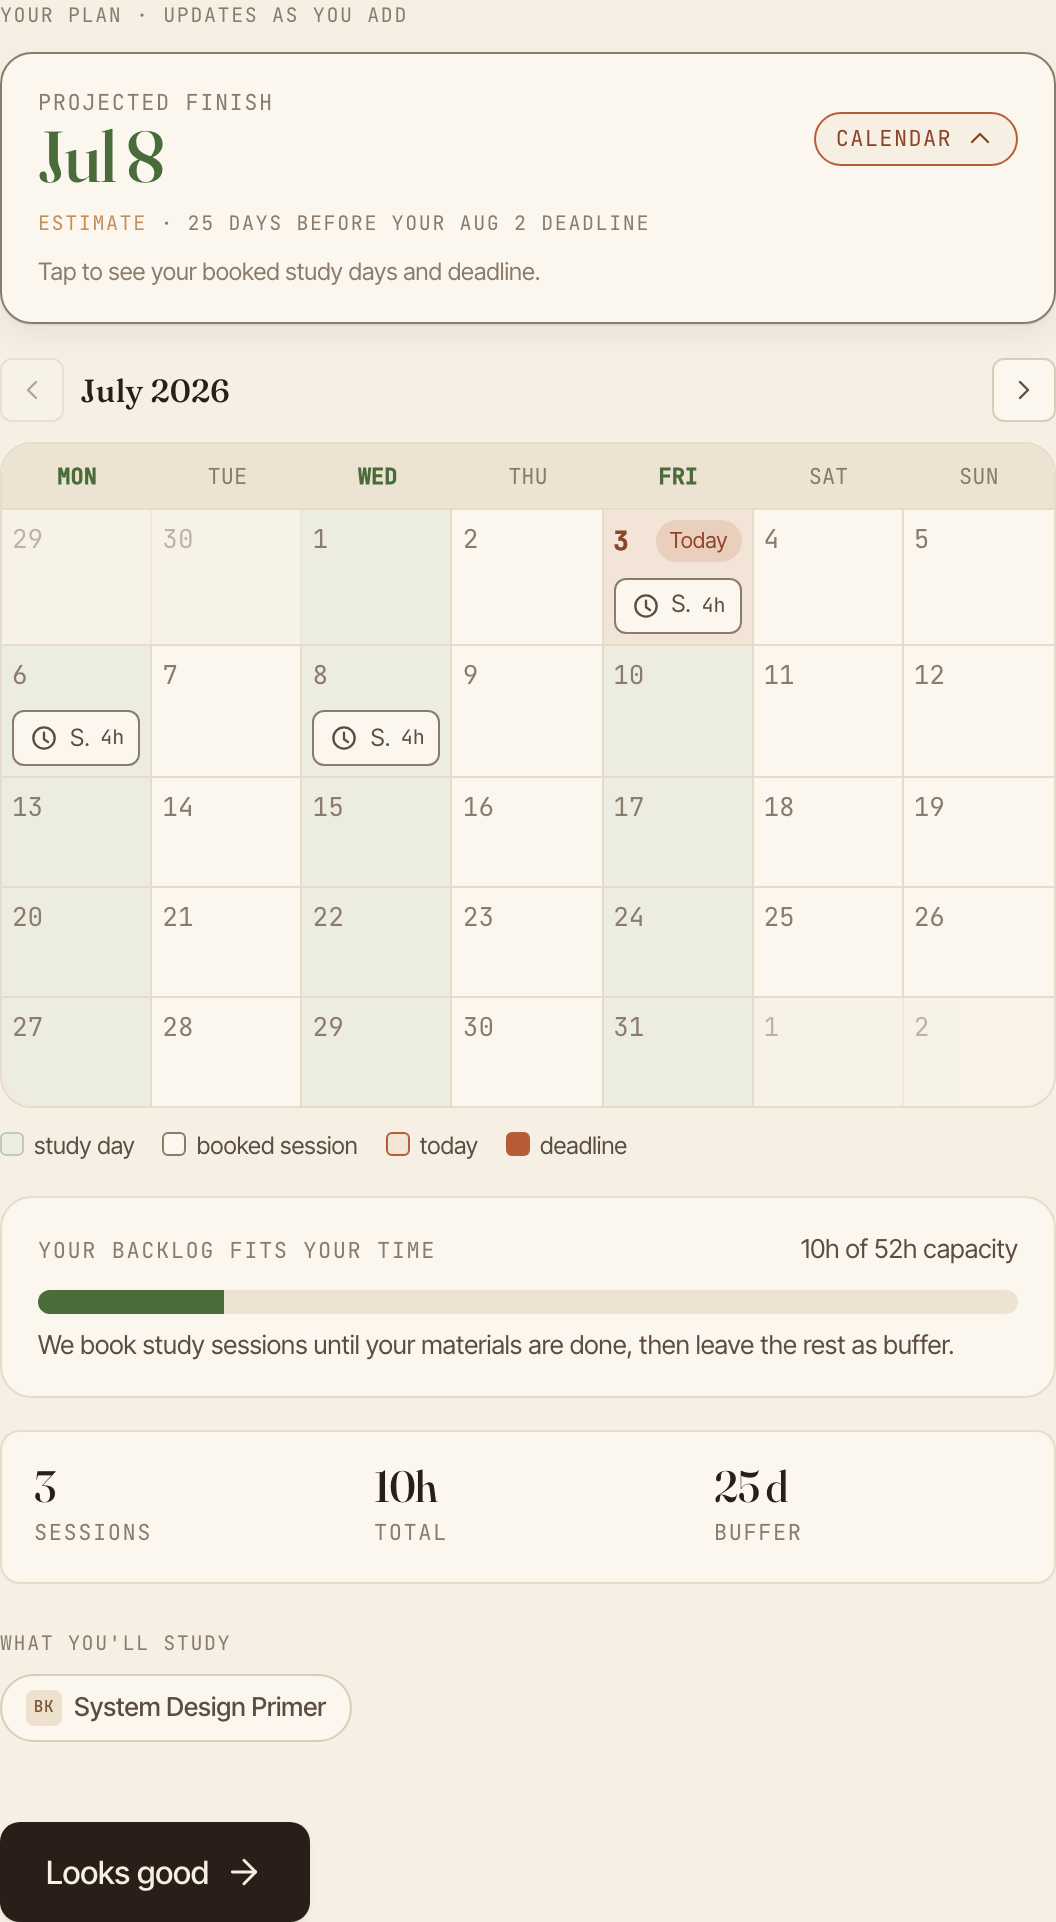
\includegraphics[width=0.85\linewidth, height=0.42\textheight, keepaspectratio]{screenshots/app_onboarding_plan.png}
\caption{Onboarding: the generated booking plan produced from the learner's deadline, weekly capacity, and materials.}
\label{fig:app-onboarding}
\end{figure}

\subsection{Study Execution: the Session Runtime}
When it is time to study, the learner starts a session from the plan and chooses the material to work on at that moment. The session runs under a timer with optional Pomodoro intervals of fifty working minutes separated by ten-minute breaks. The interval clock advances on wall-clock time, so a break that is due still arrives even after the timer has been paused. A YouTube material plays in an embedded player whose position is tracked, so that a multi-video playlist resumes at the point it reached, while an article opens in a separate tab and is timed alongside. Figure~\ref{fig:app-session} shows a session in progress.

The runtime is governed by a small state machine over idle, active, and paused states that also recognises a stale session, such as a timer left running overnight or a tab hidden for several minutes, and offers a recovery path rather than recording a spurious multi-hour session. When a session ends it records the minutes actually worked, the number of pauses, the Pomodoro blocks completed, and the position reached in each material, and this record is what later feeds the pace calibration and the progress views. A session can also be flagged as exceptional, marking an atypical day so that it does not distort the pace estimate.

\begin{figure}[htbp]
\centering
\includegraphics[width=0.85\linewidth, height=0.42\textheight, keepaspectratio]{screenshots/app_session.png}
\caption{A study session in progress, with the timer and material chosen at the start of the session.}
\label{fig:app-session}
\end{figure}

\subsection{Progress and Adaptation: Home, Week, and Replan}
Between sessions the learner sees how the plan is tracking. The Home dashboard (Figure~\ref{fig:app-home}) summarises the current state in a single view: the next booking to act on, the current and best study streak, the calibrated pace, and the projected finish date. The calibrated pace is produced by the intelligence service. The browser sends the session history to a token-verified calibration endpoint, and the Python engine returns the hierarchical-Bayesian estimate refined by the context-aware shrinkage calibrator of Equation~\eqref{eq:enriched}, together with per-role multipliers. The projection and the streak, by contrast, are computed in the browser from the local event log.

\begin{figure}[htbp]
\centering
\includegraphics[width=0.85\linewidth, height=0.42\textheight, keepaspectratio]{screenshots/app_home.png}
\caption{The Home dashboard: up-next booking, streak, calibrated pace, and projected finish date.}
\label{fig:app-home}
\end{figure}

The Week view (Figure~\ref{fig:app-week}) reports a single verdict for the week, ahead, on track, or behind, above a daily-minutes chart and a burn-up projection. The burn-up plots the cumulative minutes actually logged against the planned ramp and overlays the Gaussian-process mean with its 95\% band, falling back to an analytic estimate while fewer than five sessions have accumulated so that the early projection stays stable (Section~4.2). The point at which the band crosses the target line is the projected completion, read against the deadline.

\begin{figure}[htbp]
\centering
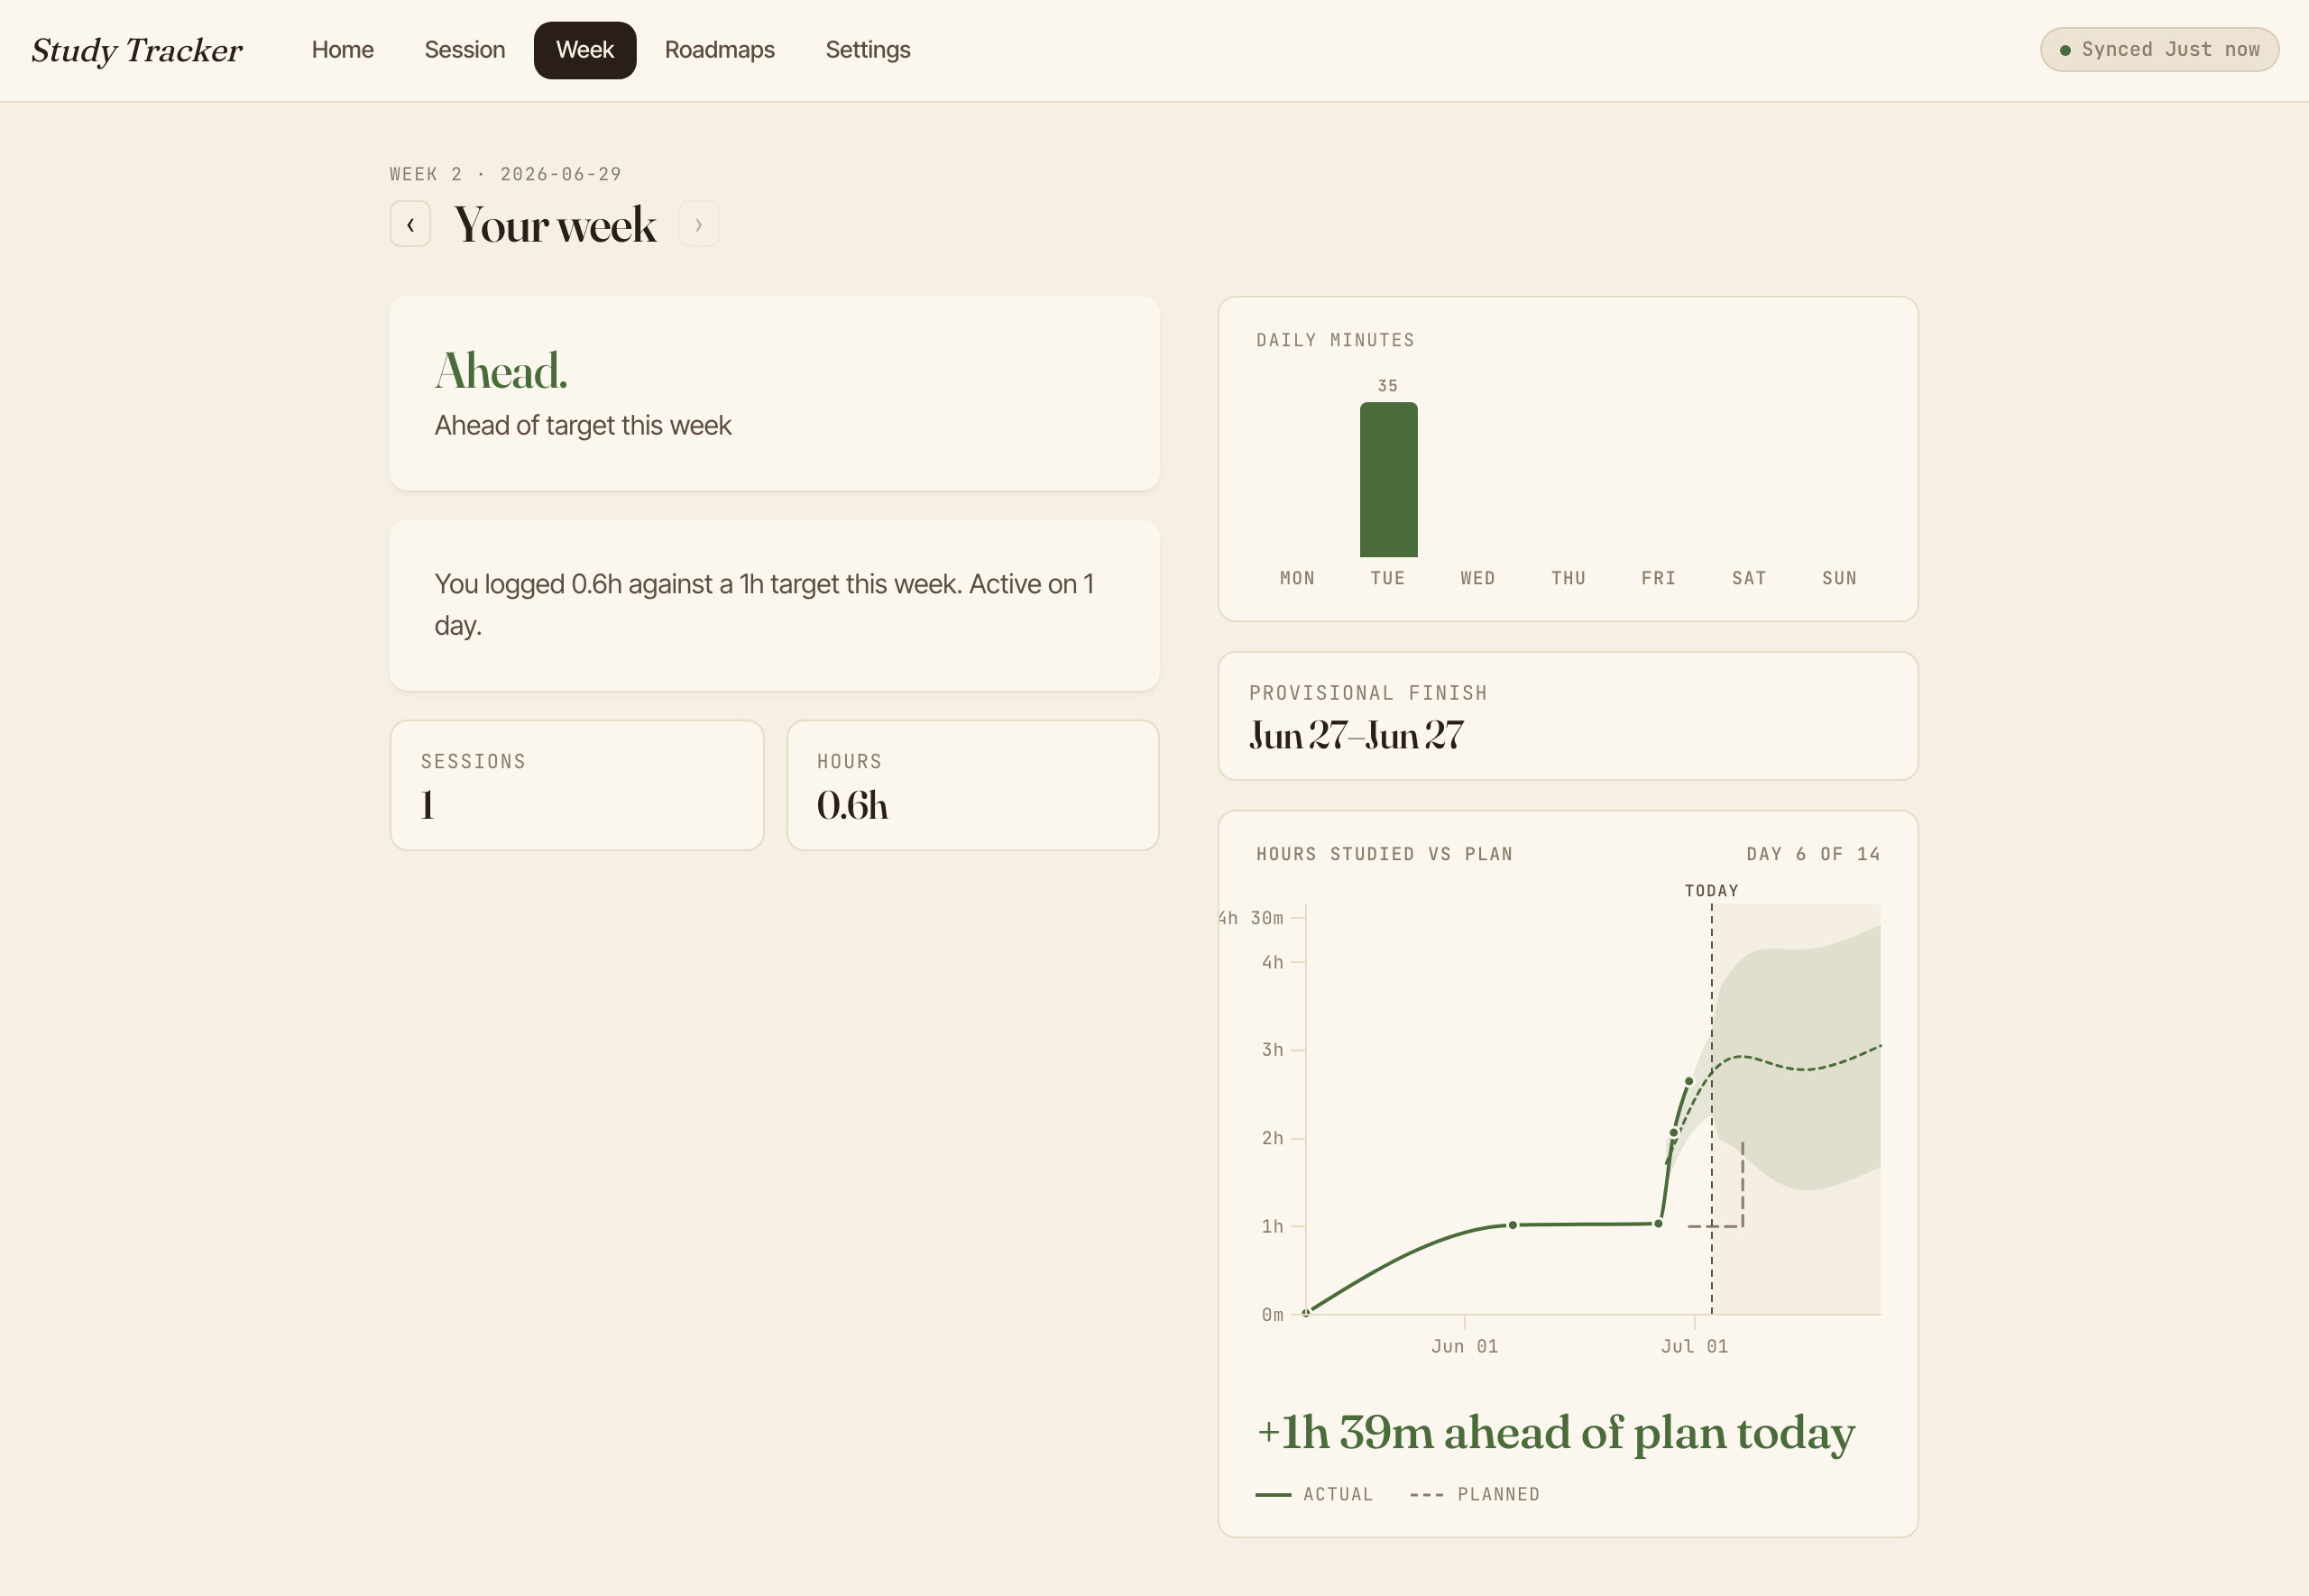
\includegraphics[width=0.85\linewidth, height=0.42\textheight, keepaspectratio]{screenshots/app_week.png}
\caption{The Week view: the week's verdict, the daily-minutes chart, and the burn-up projection.}
\label{fig:app-week}
\end{figure}

When realised pace diverges from the plan, the system does not silently rewrite the schedule. Change detection runs server-side on the same calibration call, and a divergence surfaces as a recalibration prompt that the learner can accept, acknowledge, or defer; the plan is changed only on the learner's instruction, which keeps the loop open (Section~4.1). The Replan screen (Figure~\ref{fig:app-replan}) offers three independent levers for that change: extend or shorten the deadline, raise or lower the weekly hours, or drop and trim materials. Each lever shows its effect on the projected finish date as it is moved, so the trade is visible before it is committed. Confirming a replan re-lays the bookings and records a \texttt{RoadmapReplanned} event that preserves the plan's identity, so its history remains intact.

\begin{figure}[htbp]
\centering
\includegraphics[width=0.85\linewidth, height=0.42\textheight, keepaspectratio]{screenshots/app_replan.png}
\caption{The Replan screen: three levers to adjust the plan when the projection diverges from the deadline.}
\label{fig:app-replan}
\end{figure}

\subsection{Plan Lifecycle: the Roadmap Calendar and Roadmaps Dashboard}
A plan is more than its current week. The Roadmap calendar (Figure~\ref{fig:app-roadmap}) shows the whole plan as a month grid, with study days tinted and each booking placed on its day and coloured by material role. Selecting a day opens a sheet in which the learner can add, edit, or clear a booking and mark how far through a material they have reached. A booking's status, whether unstarted, in progress, completed, trimmed, or interrupted, is derived from the logged sessions rather than stored, so it stays consistent with what actually happened.

\begin{figure}[htbp]
\centering
\includegraphics[width=0.85\linewidth, height=0.42\textheight, keepaspectratio]{screenshots/app_roadmap.png}
\caption{The Roadmap calendar: the plan shown as a month grid of bookings.}
\label{fig:app-roadmap}
\end{figure}

The Roadmaps dashboard (Figure~\ref{fig:app-roadmaps}) tracks plans across their lifecycle. The active plan is shown with its date range and progress, an unfinished onboarding draft is offered for resumption, and completed or abandoned plans are kept in a history that can be reopened read-only. Because a replan preserves the plan's identity, a plan and its successive replans collapse into a single entry rather than appearing as several unrelated plans.

\begin{figure}[htbp]
\centering
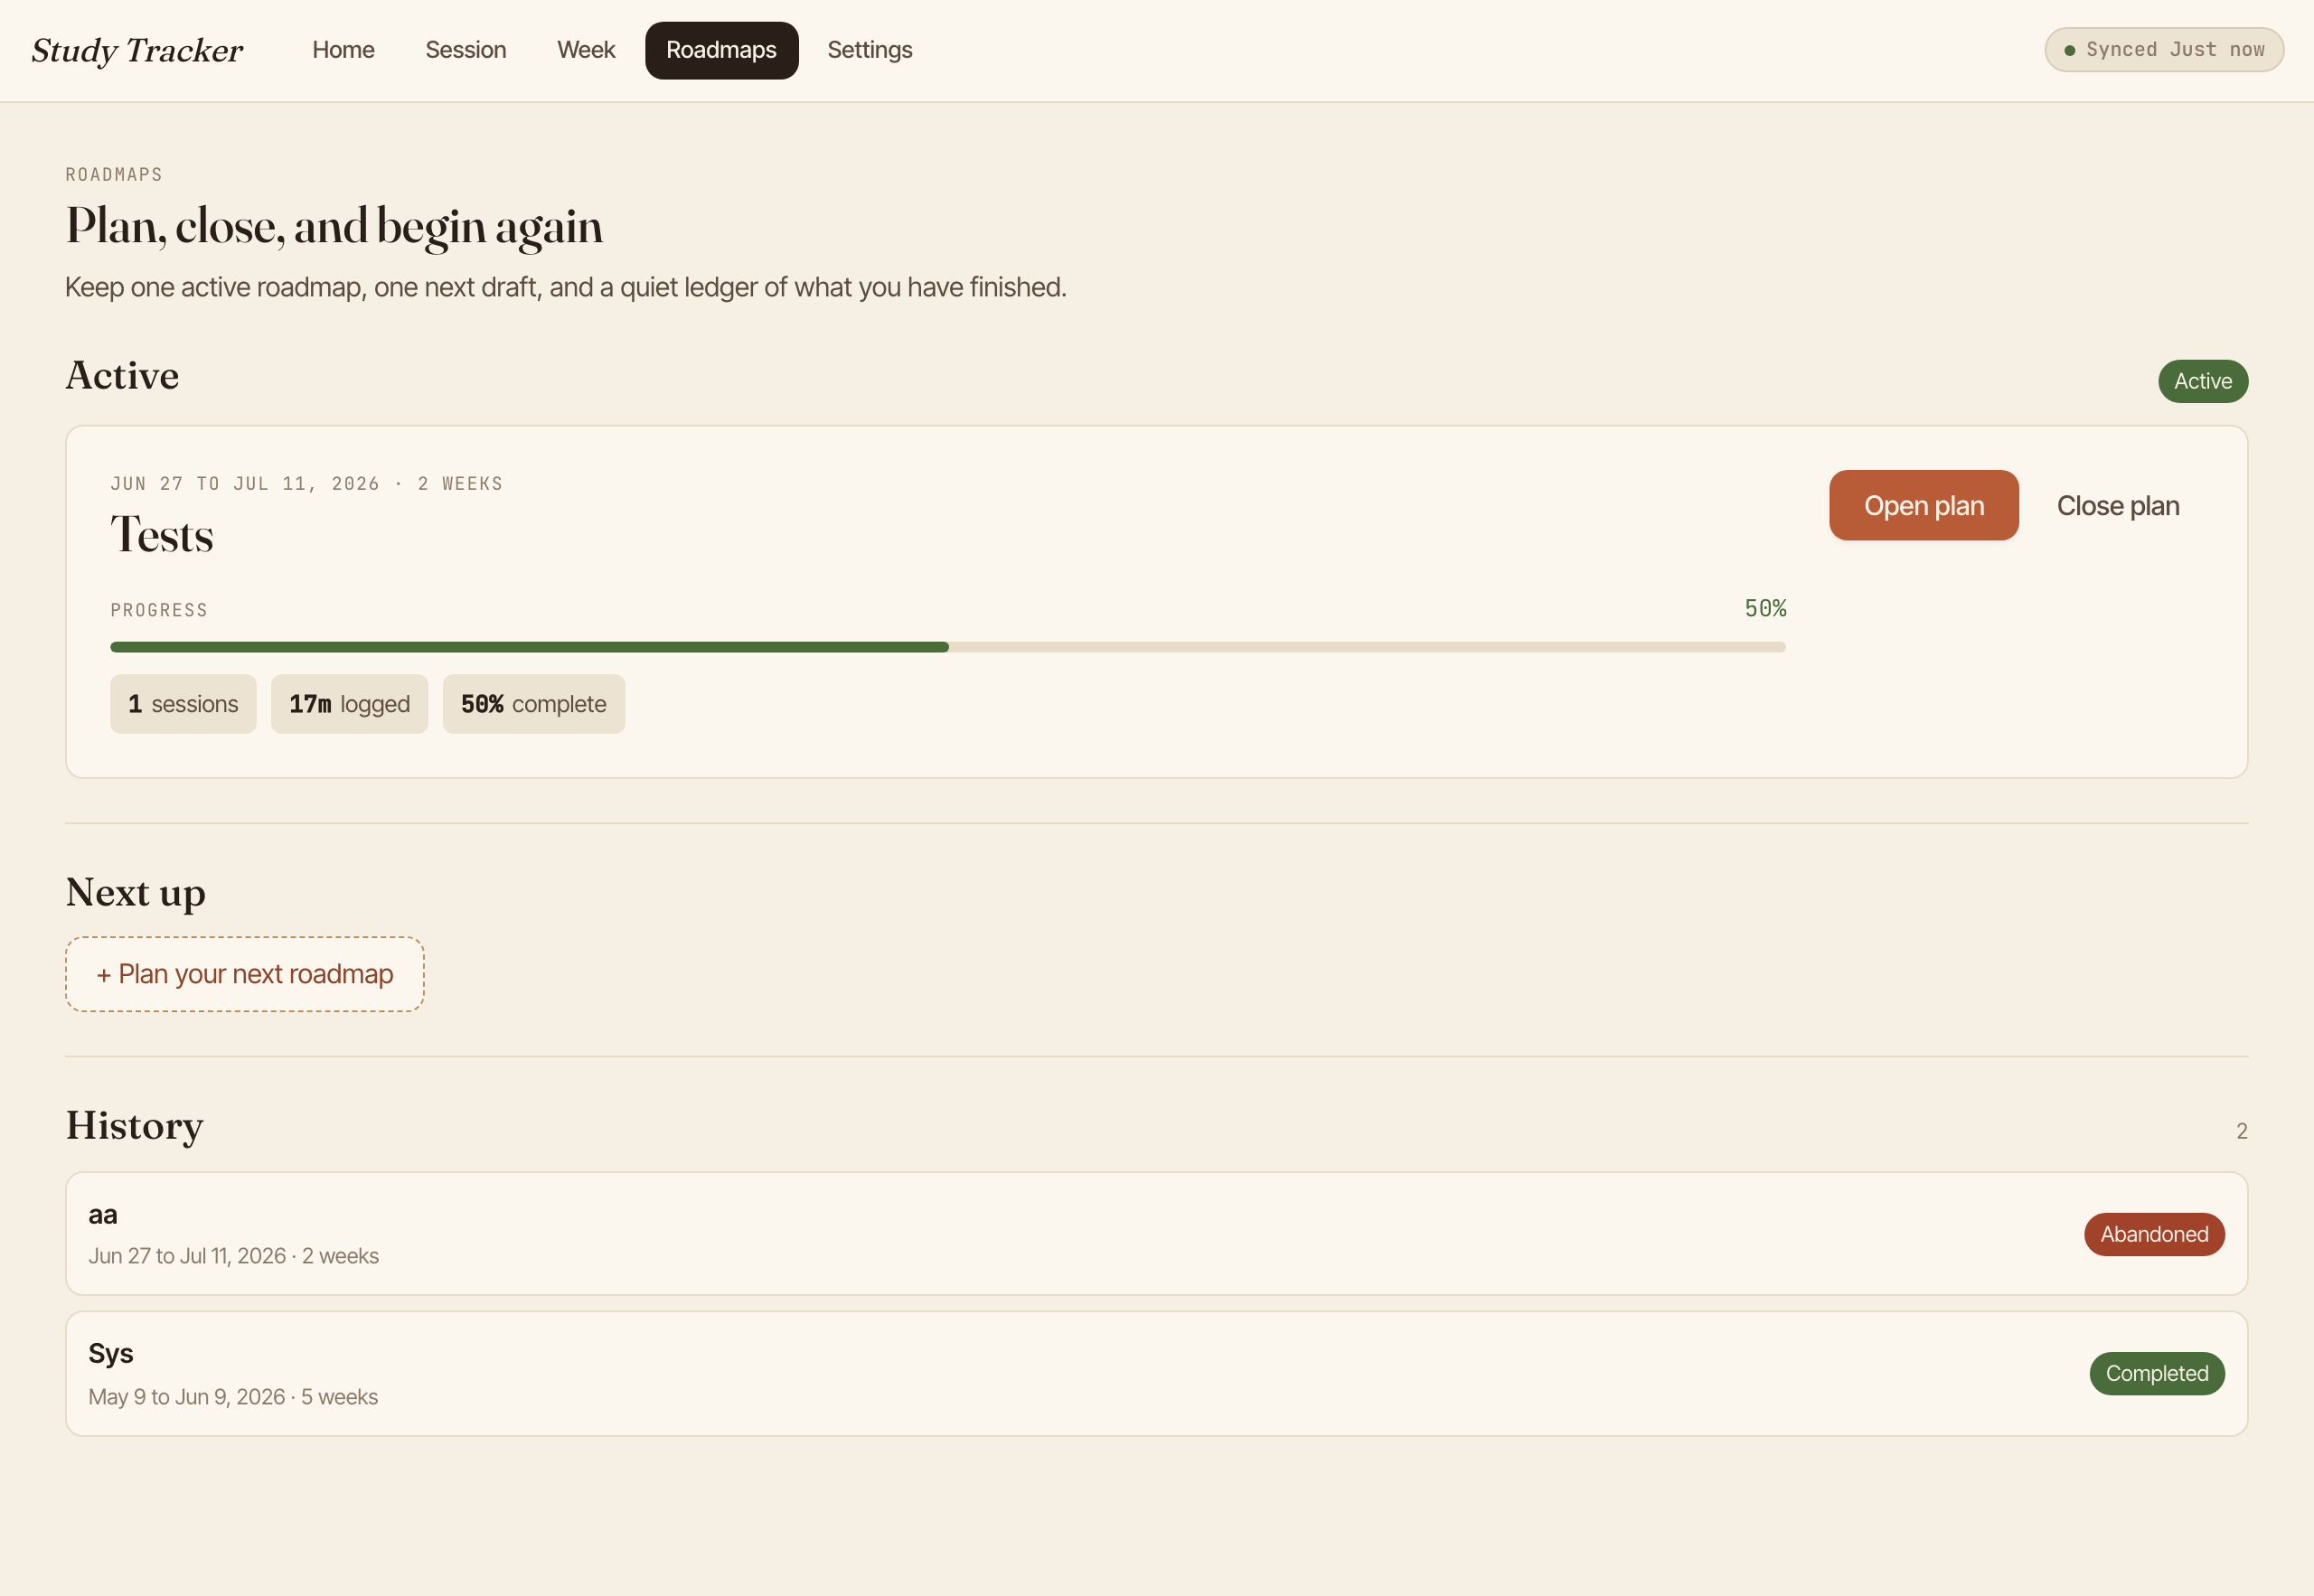
\includegraphics[width=0.85\linewidth, height=0.42\textheight, keepaspectratio]{screenshots/app_roadmaps.png}
\caption{The Roadmaps dashboard: the active plan, drafts, and history over their lifecycle.}
\label{fig:app-roadmaps}
\end{figure}

\subsection{The Local-First Data Architecture}
The four capabilities above rest on a local-first, event-sourced data layer. Every action the learner takes is recorded as an immutable event in a log held in the browser's IndexedDB, and every view, whether a dashboard, the calendar, or a projection, is derived by replaying that log rather than by reading mutable records. Because the log is local, the core loop stays usable without a network connection: reads and writes complete against the local store and reconcile with the cloud when a connection returns. Each signed-in learner has a separate local database keyed by their identity, so two accounts sharing a browser never see each other's data and neither loses its history on sign-out.

Durability to the cloud is provided by a write-ahead queue. Events are enqueued locally and flushed to a Supabase table, and a periodic snapshot of the log is uploaded to object storage, so that a new device restores the full history from the snapshot and then replays only the events recorded since it. In Phase~1 the plan's own events, its creation, its bookings, and any replan, synchronise to the cloud through this queue, while extending the same durability to the stream of events emitted during a live study session is a hardening task carried into Phase~II. The division of computation between this client and the intelligence service follows the architecture of Section~4.5 and Figure~\ref{fig:arch-revised}: model fitting over accumulated history runs in the service, and every view derived from the local log runs in the browser.
